\documentclass[12pt,a4paper]{article}
\usepackage{geometry}
\usepackage[numbers]{natbib}
\usepackage{amssymb, amsmath}
\usepackage{graphicx}
\usepackage{grffile}
\graphicspath{{../Figures/}}
\usepackage{gensymb}
\usepackage[font=small]{caption}
\usepackage[utf8]{inputenc}
\usepackage[english]{babel}
\usepackage{fancyhdr}
\usepackage[raggedright]{titlesec}
\usepackage{subcaption}
\usepackage{multirow}
\usepackage{dirtytalk}
\usepackage{framed}
\usepackage[normalem]{ulem}
\usepackage[pdftex,breaklinks]{hyperref}
\hypersetup{
  colorlinks   = true, %Colours links instead of ugly boxes
  urlcolor     = green, %Colour for external hyperlinks
  linkcolor    = blue, %Colour of internal links
  citecolor   = red %Colour of citations
}


\begin{document}
\author{Katrina Ashton}


\pagestyle{fancy}
\fancyhf{}
\rhead{\thepage}
\lhead{u5586882}

\section{What I've done}
\begin{itemize}
  \item Fixed my timestamp alignment code
  \item Wrote code to change frames
  \item Evaluated estimated trajectories compared to ground truth
  \item Checked my Kabsch implementation with synthetic data, it works well with no noise
  \item Started adding to the coordinate frames section of my report
\end{itemize}

\section{Parts of report to look at}
\begin{itemize}
\item N/A
\end{itemize}

\section{Questions}
\begin{itemize}
\item 
\end{itemize}

\section{Comments}
\begin{itemize}
  \item Jean-Luc's code is fine, there was an issue with my time alignment code which I fixed this week.
  \item The control code is harder to compare to the ground truth, the fields are "timestamp x\_vel\_des y\_vel\_des vbx vby vbz vix viy viz yaw\_des". I'll either research or ask Jean Luc how to get rotation and translation from this.
  \item I created some synthetic data and then rotated and translated it to get two point clouds. My Kabsch implementation with no noise recovers this rotation and translation with error of magnitude $10^{-15}$ for both the rotation and translation. So the issue is either with the RANSAC implementation and/or the data. Or possibly numerics?
  \item In order to get everything in the same frame for the registration, I save the trajectory in the world frame. First, I define two rotation matrices: the first, $R_{c2q}$, goes from the camera frame to quadcopter frame by rotating by 45 degrees around x. This allows me to plot the trajectory of the quadcopter rather than the camera. The second, $R_{q2w}$, goes from the quadcopter frame to the world frame (using the quadcopter pose in the world frame). This is done using a rotation -90 degrees around z  and then 180 degrees around x. So for rotation $R$ and translation $t$, the update is done as follows.
  \begin{align*}
  R_q &= R_{c2q}RR_{c2q}^T \\
  t_q &= R_{c2q}t \\
  R_{t+1} &= R_tR_q \\
  t_{q+1} &= t_t + (R_{q2w}(R_q^T t_q))^T
  \end{align*}
  \item Figure \ref{f: quad3 trj} shows the trajectories in the world frame (Figure \ref{f: quad3 kabsch} for Kabsch with different inliers), Figure \ref{f: quad3 error} shows the transaltion and rotation error of each trajecory as a function of time.
  \item I think I mentioned this before, but the distance between frames is important (compare Figure \ref{f: quad3 error} to Figure \ref{f: quad3 error 30}). The trajectory plots in this report are with 40 frames skipped.
\end{itemize}

\newpage
\begin{figure}[h]
  \begin{subfigure}[t]{0.5\textwidth}
  \centering
    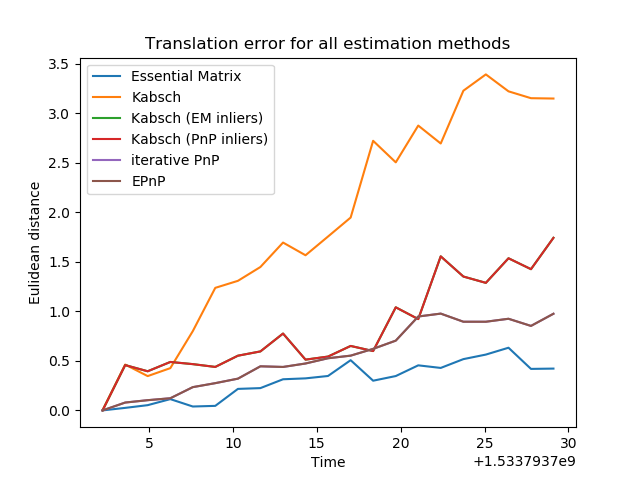
\includegraphics[width=80mm]{../quad/basic-reg-saves/et_all_40.png}
    \caption{Translation error}
  \end{subfigure} %
  ~
  \begin{subfigure}[t]{0.5\textwidth}
    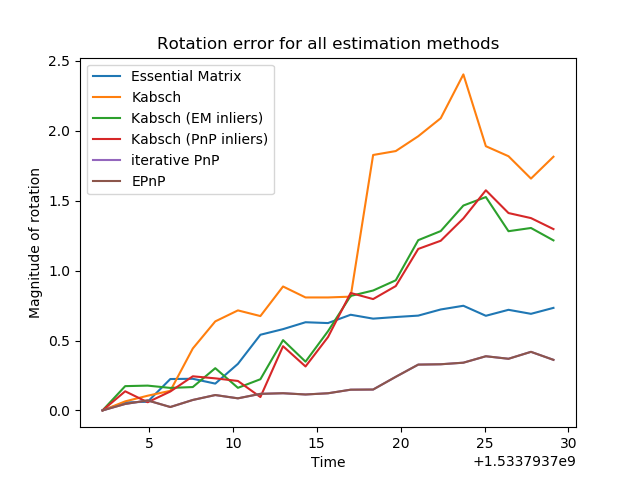
\includegraphics[width=80mm]{../quad/basic-reg-saves/eR_all_40.png}
    \caption{Rotation error}
  \end{subfigure}
  \caption{Vision error for various registration techniques with 40 frames skipped}
  \label{f: quad3 error}
\end{figure}

\begin{figure}[h]
  \begin{subfigure}[t]{0.5\textwidth}
  \centering
    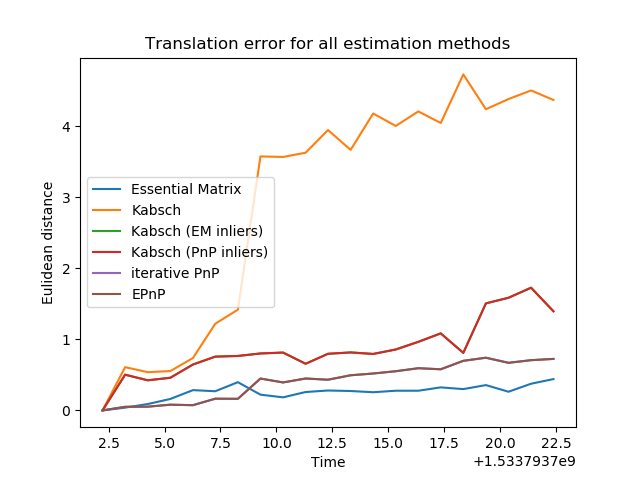
\includegraphics[width=80mm]{../quad/basic-reg-saves/et_all_30.png}
    \caption{Translation error}
  \end{subfigure} %
  ~
  \begin{subfigure}[t]{0.5\textwidth}
    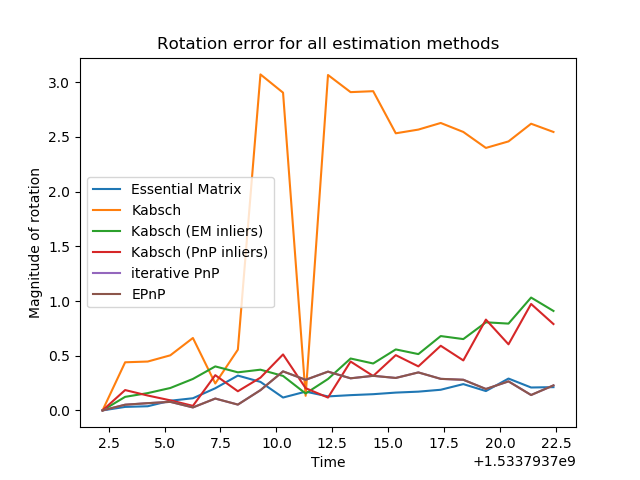
\includegraphics[width=80mm]{../quad/basic-reg-saves/eR_all_30.png}
    \caption{Rotation error}
  \end{subfigure}
  \caption{Vision error for various registration techniques with 30 frames skipped}
  \label{f: quad3 error 30}
\end{figure}

\begin{figure}[p]
\begin{subfigure}[t]{0.5\textwidth}
  \centering
    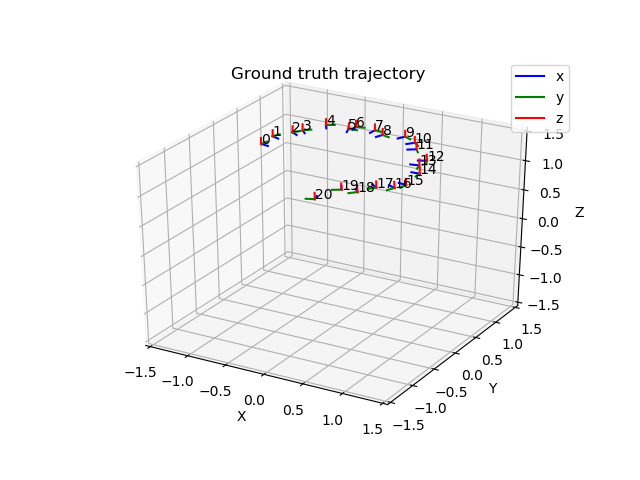
\includegraphics[width=80mm]{../quad/basic-reg-saves/rtrj_gt_40.png}
  \caption{Ground truth from Vicon}
  \end{subfigure}%
  ~
  \begin{subfigure}[t]{0.5\textwidth}
  \centering
    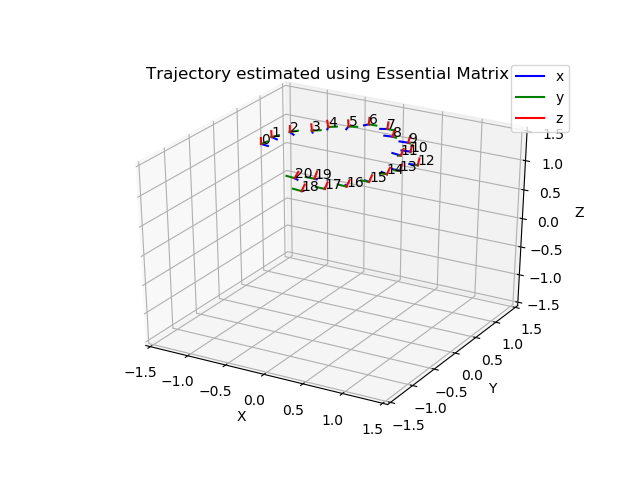
\includegraphics[width=80mm]{../quad/basic-reg-saves/rtrj_rgb_40.png}
  \caption{Estimated trajectory for Essential Matrix method, start at origin. Note axes scaling x4}
  \end{subfigure}
  \\
  \begin{subfigure}[t]{0.5\textwidth}
  \centering
    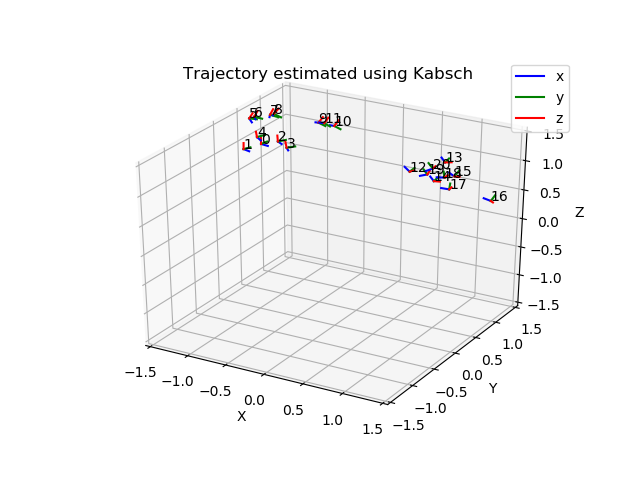
\includegraphics[width=80mm]{../quad/basic-reg-saves/rtrj_d_40.png}
  \caption{Estimated trajectory for Kabsch method, start at origin. Note axes scaling x2}
  \end{subfigure}%
  ~
  \begin{subfigure}[t]{0.5\textwidth}
  \centering
    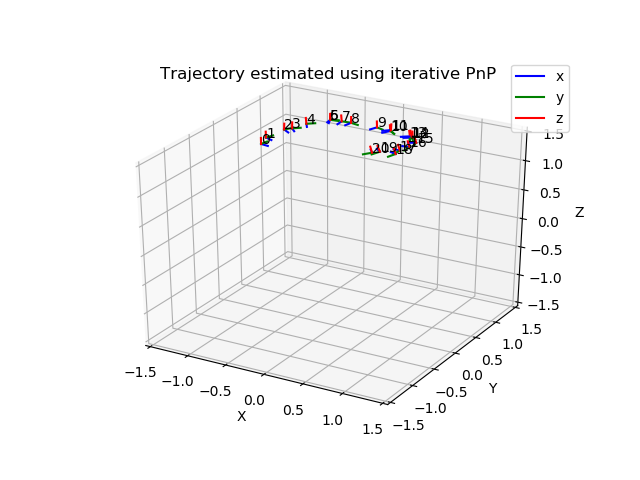
\includegraphics[width=80mm]{../quad/basic-reg-saves/rtrj_pnp_40.png}
  \caption{Estimated trajectory for PnP method, start at origin. Note axes scaling x2}
  \end{subfigure}
  \caption{Trajectory visualizations for third quad dataset}
  \label{f: quad3 trj}
\end{figure}

\begin{figure}[h]
\begin{subfigure}[t]{\textwidth}
  \centering
    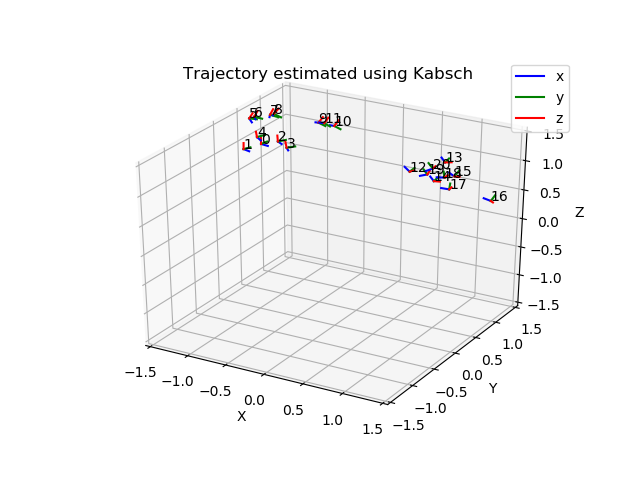
\includegraphics[width=80mm]{../quad/basic-reg-saves/rtrj_d_40.png}
  \caption{RANSAC Kabsch}
  \end{subfigure}%
  \\
  \begin{subfigure}[t]{0.5\textwidth}
  \centering
    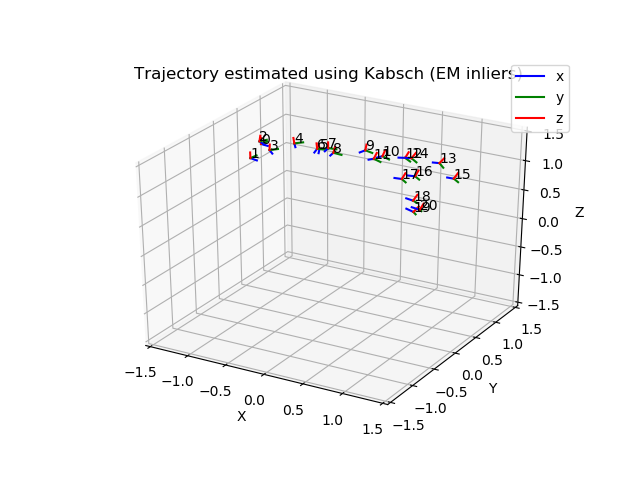
\includegraphics[width=80mm]{../quad/basic-reg-saves/rtrj_de_40.png}
  \caption{Kabsch with Essential Matrix inliers}
  \end{subfigure}%
  ~
  \begin{subfigure}[t]{0.5\textwidth}
  \centering
    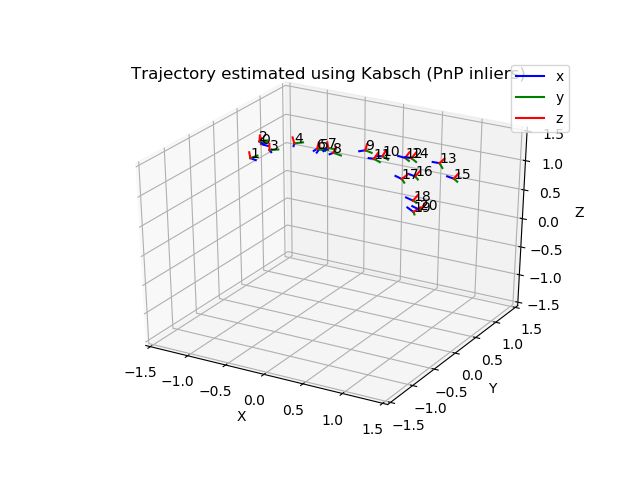
\includegraphics[width=80mm]{../quad/basic-reg-saves/rtrj_dp_40.png}
  \caption{Kabsch with PnP inliers}
  \end{subfigure}
  \caption{Trajectory visualizations for third quad dataset, Kabsch method with different inliers}
  \label{f: quad3 kabsch}
\end{figure}





\bibliographystyle{abbrvnat}
\bibliography{../Report/ENGN4217}

\end{document}